\documentclass[border=10pt]{standalone}
\usepackage{tkz-graph}
\tikzset{
  VertexStyle/.append style = { inner sep=5pt },
  EdgeStyle/.append style = {->},
}
\thispagestyle{empty}

\begin{document}
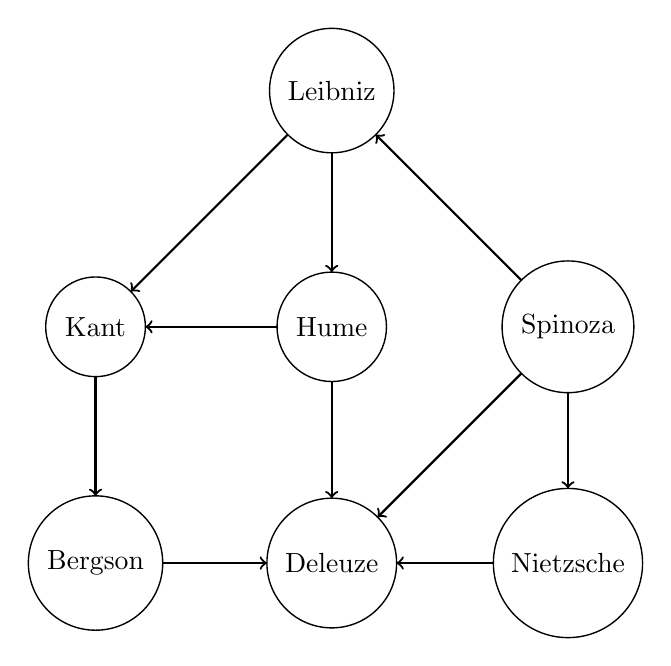
\begin{tikzpicture}
  \SetGraphUnit{3}
  \Vertex{Leibniz}
  \SO(Leibniz){Hume}
  \SOEA(Leibniz){Spinoza}
  \SOWE(Leibniz){Kant}
  \SO(Hume){Deleuze}
  \SO(Kant){Bergson}
  \SO(Spinoza){Nietzsche}

  \Edge(Spinoza)(Leibniz)
  \Edge(Leibniz)(Kant)
  \Edge(Leibniz)(Hume)

  \Edge(Kant)(Bergson)
  \Edge(Bergson)(Deleuze)
  \Edge(Spinoza)(Deleuze)
  \Edge(Hume)(Deleuze)
  \Edge(Hume)(Kant)
  \Edge(Spinoza)(Nietzsche)
  \Edge(Nietzsche)(Deleuze)
\end{tikzpicture}
\end{document}
